\ifx\allfiles\undefined
\documentclass[12pt, a4paper,oneside, UTF8]{ctexbook}
\usepackage[dvipsnames]{xcolor}
\usepackage{mathtools}   % 数学公式(mathtools 是 amsmath 的上位替代)
\usepackage{amsthm}    % 定理环境
\usepackage{amssymb}   % 更多公式符号
\usepackage{graphicx}  % 插图
%\usepackage{mathrsfs}  % 数学字体
%\usepackage{newtxtext,newtxmath}
%\usepackage{arev}
\usepackage{kmath,kerkis}
\usepackage{newtxtext}
\usepackage{bbm}
\usepackage{enumitem}  % 列表
\usepackage{geometry}  % 页面调整
%\usepackage{unicode-math}
\usepackage[colorlinks,linkcolor=black]{hyperref}

\usepackage{wrapfig}


\usepackage{ulem}	   % 用于更多的下划线格式,
					   % \uline{}下划线,\uuline{}双下划线,\uwave{}下划波浪线,\sout{}中间删除线,\xout{}斜删除线
					   % \dashuline{}下划虚线,\dotuline{}文字底部加点


\graphicspath{ {flg/},{../flg/}, {config/}, {../config/} }  % 配置图形文件检索目录
\linespread{1.5} % 行高

% 页码设置
\geometry{top=25.4mm,bottom=25.4mm,left=20mm,right=20mm,headheight=2.17cm,headsep=4mm,footskip=12mm}

% 设置列表环境的上下间距
\setenumerate[1]{itemsep=5pt,partopsep=0pt,parsep=\parskip,topsep=5pt}
\setitemize[1]{itemsep=5pt,partopsep=0pt,parsep=\parskip,topsep=5pt}
\setdescription{itemsep=5pt,partopsep=0pt,parsep=\parskip,topsep=5pt}

% 定理环境
% ########## 定理环境 start ####################################
\theoremstyle{definition}
\newtheorem{defn}{\indent 定义}[section]

\newtheorem{lemma}{\indent 引理}[section]    % 引理 定理 推论 准则 共用一个编号计数
\newtheorem{thm}[lemma]{\indent 定理}
\newtheorem{corollary}[lemma]{\indent 推论}
\newtheorem{criterion}[lemma]{\indent 准则}

\newtheorem{proposition}{\indent 命题}[section]
\newtheorem{example}{\indent \color{SeaGreen}{例}}[section] % 绿色文字的 例 ,不需要就去除\color{SeaGreen}{}
\newtheorem*{rmk}{\indent \color{red}{注}}

% 两种方式定义中文的 证明 和 解 的环境:
% 缺点:\qedhere 命令将会失效【技术有限,暂时无法解决】
\renewenvironment{proof}{\par\textbf{证明.}\;}{\qed\par}
\newenvironment{solution}{\par{\textbf{解.}}\;}{\qed\par}

% 缺点:\bf 是过时命令,可以用 textb f等替代,但编译会有关于字体的警告,不过不影响使用【技术有限,暂时无法解决】
%\renewcommand{\proofname}{\indent\bf 证明}
%\newenvironment{solution}{\begin{proof}[\indent\bf 解]}{\end{proof}}
% ######### 定理环境 end  #####################################

% ↓↓↓↓↓↓↓↓↓↓↓↓↓↓↓↓↓ 以下是自定义的命令  ↓↓↓↓↓↓↓↓↓↓↓↓↓↓↓↓

% 用于调整表格的高度  使用 \hline\xrowht{25pt}
\newcommand{\xrowht}[2][0]{\addstackgap[.5\dimexpr#2\relax]{\vphantom{#1}}}

% 表格环境内长内容换行
\newcommand{\tabincell}[2]{\begin{tabular}{@{}#1@{}}#2\end{tabular}}

% 使用\linespread{1.5} 之后 cases 环境的行高也会改变,重新定义一个 ca 环境可以自动控制 cases 环境行高
\newenvironment{ca}[1][1]{\linespread{#1} \selectfont \begin{cases}}{\end{cases}}
% 和上面一样
\newenvironment{vx}[1][1]{\linespread{#1} \selectfont \begin{vmatrix}}{\end{vmatrix}}

\def\d{\textup{d}} % 直立体 d 用于微分符号 dx
\def\R{\mathbb{R}} % 实数域
\def\N{\mathbb{N}} % 自然数域
\def\C{\mathbb{C}} % 复数域
\def\Z{\mathbb{Z}} % 整数环
\def\Q{\mathbb{Q}} % 有理数域
\newcommand{\bs}[1]{\boldsymbol{#1}}    % 加粗,常用于向量
\newcommand{\ora}[1]{\overrightarrow{#1}} % 向量

% 数学 平行 符号
\newcommand{\pll}{\kern 0.56em/\kern -0.8em /\kern 0.56em}

% 用于空行\myspace{1} 表示空一行 填 2 表示空两行  
\newcommand{\myspace}[1]{\par\vspace{#1\baselineskip}}

%s.t. 用\st就能打出s.t.
\DeclareMathOperator{\st}{s.t.}

%罗马数字 \rmnum{}是小写罗马数字, \Rmnum{}是大写罗马数字
\makeatletter
\newcommand{\rmnum}[1]{\romannumeral #1}
\newcommand{\Rmnum}[1]{\expandafter@slowromancap\romannumeral #1@}
\makeatother
\begin{document}
	% \title{{\Huge{\textbf{$Partial \,\, Differential \,\, Equations$}}}\footnote{参考书籍:\\
			\hspace*{4em} \textbf{《Partial Differential Equations》 -- Lawrence C. Evans} \\
			\hspace*{4em} \textbf{《Partial Differential Equations》 -- Fritz John} \\
			\hspace*{4em} \textbf{《数学物理方程讲义 (第二版)》--  姜礼尚、陈亚浙、刘西垣、易法槐} 
			}}
\author{$-TW-$}
\date{\today}
\maketitle                   % 在单独的标题页上生成一个标题

\thispagestyle{empty}        % 前言页面不使用页码
\begin{center}
	\Huge\textbf{序}
\end{center}


\vspace*{3em}
\begin{center}
	\large{\textbf{天道几何,万品流形先自守;}}\\
	
	\large{\textbf{变分无限,孤心测度有同伦。}}
\end{center}

\vspace*{3em}
\begin{flushright}
	\begin{tabular}{c}
		\today \\ \small{\textbf{长夜伴浪破晓梦,梦晓破浪伴夜长}}
	\end{tabular}
\end{flushright}


\newpage                      % 新的一页
\pagestyle{plain}             % 设置页眉和页脚的排版方式(plain:页眉是空的,页脚只包含一个居中的页码)
\setcounter{page}{1}          % 重新定义页码从第一页开始
\pagenumbering{Roman}         % 使用大写的罗马数字作为页码
\tableofcontents              % 生成目录

\newpage                      % 以下是正文
\pagestyle{plain}
\setcounter{page}{1}          % 使用阿拉伯数字作为页码
\pagenumbering{arabic}
\setcounter{chapter}{0}    % 设置 -1 可作为第零章绪论从第零章开始 
	\else
	\fi
	%  ############################ 正文部分
\chapter{The Single First-Order Equation}

\section{一阶线性方程的特征线解法}
	对于\textbf{波动方程}来说, 经典的解题方法有两类:\textbf{分离变量法$\&$ 特征线法}. 这两类方法也可以应用于除波动方程外的很多PDE. 这一节我们以\textbf{一阶线性方程}为例, 引出\textbf{特征线}的概念. 
	
\subsection{一阶常系数线性方程}
	首先先来考虑最简单的情形:在区域$\R \times (0 , \infty)$ 上求解Cauchy问题:
	\begin{equation}
		\begin{cases}
			\dfrac{\partial \rho}{\partial t} + a \dfrac{\partial \rho}{\partial x} = 0 \\
			\rho(x , 0) = \rho_0(x)
		\end{cases}\label{1.1}
	\end{equation}
	
	\vspace*{1em}
	
	对于该问题, 给出\textbf{特征线}的定义. 
	\begin{defn}\label{def 1.1.1}
		我们称下列ODE初值问题
		\begin{align*}
			\begin{cases}
				\dfrac{dx}{dt} = a \\
				x(0) = c
			\end{cases}
		\end{align*}
		的解$x(t , c) = at + c$ 为方程(\ref{1.1})的\underline{\textcolor{blue}{\textbf{特征线}}}, 其中$c \in \R$ 为常数. 
			
		\vspace*{3em}
		
		\begin{rmk}
			\textbf{“特征线”}的含义如下:\\
			沿着特征线$x = x(t , c)$, 待求函数表达式为$\rho = \rho\Big( x(t , c) , t \Big)$, $\st$
			\[ \frac{d\rho}{dt} = \frac{\partial \rho}{\partial t} + \frac{\partial \rho}{\partial x} \cdot \frac{dx}{dt} = \rho_t + a\rho_x = 0 \]
			即$\rho(x , t)$ 在特征线$x = x(t , c)$ 上恒为常数. \\
			故只需知道特征线上一点取值即可得到整条线上的函数值. 而在特征线的起点$x = c , \,\, t = 0$ 处, 
			\[ \rho\Big( x(0 , c) , 0 \Big) = \rho(c , 0) = \rho_0(c) \]
			于是在特征线$x = x(t , c)$ 上, 
			\[ \rho\Big( x(t , c) , t \Big) = \rho(at + c , c) = \rho_0(c) \]
			根据$x = at + c$, 解得$c = x - at$, 代入上式, 得到$\rho(x , t)$ 的解
			\[ \rho(x , t) = \rho_0(x - at) , \,\, \forall (x , t) \in \R \times (0 , \infty) \]
		\end{rmk}
	\end{defn}
	
\vspace*{5em}
	
\subsection{一阶变系数线性方程}
	更一般地, 我们考虑变系数方程
	\begin{align}
		\frac{\partial \rho}{\partial t} &+ \frac{\partial}{\partial x} \Big( v(x) \cdot \rho \Big) = 0 \\
		\Leftrightarrow \,\, \frac{\partial \rho}{\partial t} &+ v(x) \frac{\partial \rho}{\partial x} + v^{'}(x) \rho = 0 \label{1.3}
	\end{align}
	
	\vspace*{1em}
	
	类似地, 对于该变系数问题, 同样给出\textbf{特征线}的定义. 
	
	\begin{defn}\label{def 1.1.2}
		设曲线$x = x(t , c)$ 满足
		\begin{align*}
			\begin{cases}
				\dfrac{dx}{dt} = v\Big( x(t) \Big) \\
				x(0) =c
			\end{cases}
		\end{align*}
		这条积分曲线$x = x(t , c)$ 称为方程(\ref{1.3}) 的\underline{\textcolor{blue}{\textbf{特征线}}}, 其中$c \in \R$ 为常数. 沿着特征线$x = x(t , c)$, 待求函数$\rho = \rho\Big( x(t , c) , t \Big)$ 满足:
		\begin{align}
			\begin{cases}
				\dfrac{d \rho}{dt} = - v^{'}\Big( x(t , c) \Big) \cdot \rho \\
				\rho \Big( x(0 , c) , 0 \Big) = \rho(c , 0) = \rho_0(c)
			\end{cases}\label{1.4}
		\end{align}
		
		\vspace*{2em}
		
		\begin{rmk}
			 事实上, 此处我们已经将PDE问题(\ref{1.3}) 转化为了求解ODE问题(\ref{1.4}). 但在处理积分时要留意, 方程(\ref{1.4}) 中等号右端函数$v^{'}$ 的自变量为$x(t , c)$ 而非$t$, 因此要进行变量替换, 即
			 \begin{align*}
			 	\frac{d \rho}{\rho} &= - v^{'} \Big( x(t , c) \Big) dt \\
			 	\ln \rho \Big( x(t , c) , t \Big) - \ln \rho_0(c) &= \int_{0}^t - v^{'} \Big( x(\tau , c) \Big) \, d\tau \\
			 	&= \int_{c}^{x(t , c)} - v^{'} \Big( x(t , c) \Big) \cdot \dfrac{1}{\dfrac{dx}{d\tau}} \cdot dx
			 \end{align*}
		 	由于特征线方程满足
		 	\[ \frac{dx}{dt} = v \Big( x(t , c) \Big) \]
		 	因此
		 	\begin{align*}
		 		\ln \rho \Big( x(t , c) , t \Big) - \ln \rho_0(c) 
		 		&= \int_{c}^{x(t , c)} - v^{'} \Big( x(t , c) \Big) \cdot \dfrac{1}{\dfrac{dx}{d\tau}} \cdot dx \\
		 		&= \int_{c}^{x(t , c)} \frac{- v^{'} \Big( x(t , c) \Big)}{v \Big( x(t , c) \Big)} \, dx \\
		 		&= -\ln v \Big( x(t , c) \Big) + \ln v(c)
		 	\end{align*}
	 		从而容易得到特征线$x = x(t , c)$ 上函数$\rho = \rho\Big( x(t , c) , t \Big)$为
	 		\[ \rho\Big( x(t , c) , c \Big) = \rho_0(c) \cdot \frac{v(c)}{v \Big( x(t , c) \Big)}\]
	 		从特征线方程$x = x(t , c)$ 中解出$c = \varphi(x , t)$, 代入上式, 解得
	 		\[ \rho(x , t) = \rho_0\Big( \varphi(x , t) \Big) \cdot \frac{v \Big( \varphi(x , t) \Big)}{v(x)} \]
	 		可以验证, 上述表达式确实是方程(\ref{1.3}) 的解. 
		\end{rmk}
	\end{defn}

\newpage

\subsection{一阶线性方程的特征线解法}
	下面对前两个小节所给出的\textbf{特征线法}进行总结归纳, 大致分为以下步骤:
	
	\vspace*{1em}
	
	\begin{enumerate}
		\item 求特征线$x = x(t , c)$. 
		
		\vspace*{1em}
		
		\item 沿特征线$x = x(t , c)$, 将原方程化为关于$\rho = \rho \Big( x(t , c) , t \Big)$ 的ODE方程(其中$c \in \R$ 为参数), 并求出$\rho = u(t , c)$. 
		
		\vspace*{1em}
		
		\item 从特征线方程$x = x(t , c)$ 中解出$c = \varphi(x , t)$, 代入$\rho = u(t , c)$ 中, 解得$\rho(x , t) = u \Big( t , \varphi(x , t) \Big)$.
	\end{enumerate}
	
	\vspace*{4em}
	
	下面给出一个实例. 
	\begin{example}\label{ex 1.1.1}
		求下列Cauchy问题的解. 
		\begin{align*}
			\begin{cases}
				\dfrac{\partial u}{\partial t} + (x + t) \dfrac{\partial u}{\partial x} + u = x , \,\, x \in \R , \,\, t > 0 \\
				u(x , 0) = x
			\end{cases}
		\end{align*}
		
		\vspace*{2em}
		
		\begin{solution}
			\begin{enumerate}
				\item[\textbf{Step 1}]. 求特征线. 特征方程
				\begin{align*}
					\begin{cases}
						\dfrac{dx}{dt} = x + t \\
						x(0) = c
					\end{cases}
				\end{align*}
				的解为
				\[ x = x(t) = e^t (1 + c) - (1 + t) \]
				
				\vspace*{2em}
				
				\item[\textbf{Step 2}]. 令$U(t) = u\Big( x(t) , t \Big)$, then
				\begin{align*}
					\begin{cases}
						\dfrac{dU}{dt} = x(t) - u\Big( x(t) , t \Big) = -U(t) + e^t (1 + c) - (1 + t) \\
						U(0) = u\Big( x(0), 0 \Big) = u(c , 0) = c
					\end{cases}
				\end{align*}
				解得
				\[ U(t) = u \Big( x(t) , t \Big) = \frac{1}{2}(c + 1) e^t + \frac{1}{2}(c - 1) e^{-t} - t \]
				
				\item[\textbf{Step 3}]. 从特征线方程$x = e^t (1 + c) - (1 + t)$ 中, 解得
				\[ c = (x + t + 1)e^{-t} - 1 \]
				代入$u \Big( x(t) , t \Big)$ 中, 得到
				\[ u(x , t) = \frac{1}{2} e^{-2t} (x + t + 1) - e^{-t} + \frac{1}{2}(x - t + 1) \]
			\end{enumerate}
		\end{solution}
	\end{example}

\newpage

\section{Quasi-Linear Equations}
	这一节我们将会把\textbf{线性方程}中的\textbf{特征线法}拓展到更一般的\textbf{Quasi-Linear} 方程中, 并将给出\textbf{Integral Surfaces (积分曲面)}等概念. 此处我们为了简化问题, 均讨论\textbf{含2个自变量的一阶Quasi-Linear方程}, 即
	\begin{align}
		a(x , y , u) u_x + b(x , y , u)u_y = c(x , y , u) \label{1.5}
	\end{align}
	
\subsection{Integral Surfaces}
	为了直观地理解方程(\ref{1.5}), 我们不妨令$z = u(x , y)$ 代表$\R^3$ 中的曲面, 方程(\ref{1.5}) 可化为
	\[ (a , b , c) \cdot (u_x , u_y , -1) = 0 \]
	根据\textbf{外法向的定义 (\ref{def B.1.1})}, $(u_x , u_y , -1)$ 即为曲面$z = u(x , y)$ 在各点处的外法向. 于是对于$\R^3$ 中向量场$(a , b , c)$, 其与曲面$z = u(x , y)$ 在各点处的法向量垂直. 
	
	\vspace*{3em}
	
	\hspace*{-1.85em}从而我们的问题可由\textbf{“求解方程(\ref{1.5})”}, 转化为:
	\begin{center}
		\textbf{对于$\R^3$ 中的向量场$(a , b , c)$, 我们要找到一个曲面$z = u(x , y)$, \\
			$\st$ 曲面上每个点的切线均平行于$(a , b , c)$}.
	\end{center}
	
	\vspace*{1em}
	
	\begin{figure}[thbp!]
		\centering
		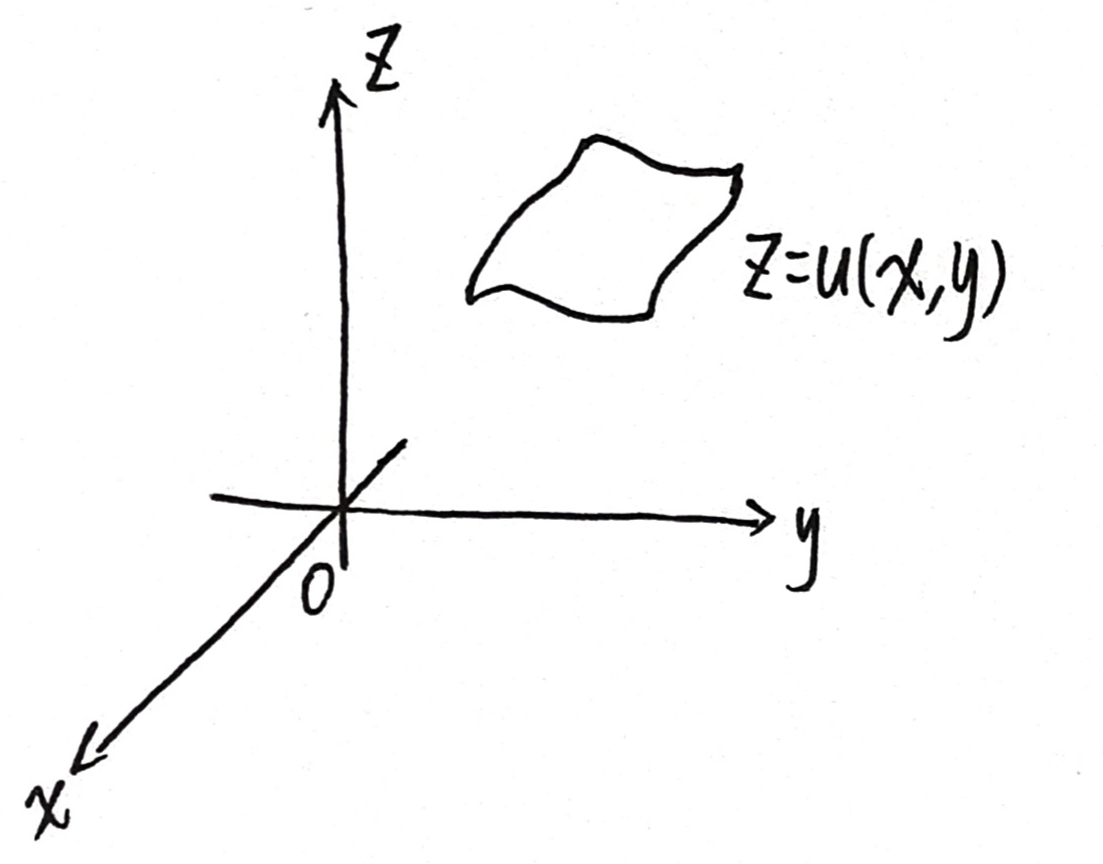
\includegraphics[width=0.3\linewidth]{figure/1.2-1}
		\caption{曲面$z = u(x , y)$}
		\label{pic : 1.2-1} % 添加图像引用标签
	\end{figure}
	
	\hspace*{-1.85em}由此, 引出\textbf{Integral Surfaces} 的概念. 
	
	\begin{defn}\label{def 1.2.1}
		Surfaces corresponding to solutions of a P.D.E. are called \underline{\textcolor{blue}{\textbf{integral surfaces}}} of the P.D.E.
	\end{defn}

\newpage

\subsection{Characteristic Curves}
	为了求解\textbf{Quasi-Linear Equations}, 我们来拓展\textbf{Def \ref{def 1.1.1}}及\textbf{Def \ref{def 1.1.2}} 中关于\textbf{特征线}的概念. Assume $a , b , c \in C^1(\Omega)$, where $\Omega \subset \R^3$ is a bounded region. 对于方程(\ref{1.5}), 
	\[ a(x , y , u) u_x + b(x , y , u)u_y = c(x , y , u) \]
	我们给出\textbf{特征线}的定义. 
	
	\vspace*{1em}
	
	\begin{defn}\label{def 1.2.2}
		设曲线$\gamma : (x(t) , y(t) , z(t)) \subset \R^3$. 若曲线$\gamma$ 满足ODE方程组
		\begin{align}
			\begin{cases}
				\dfrac{dx}{dt} = a(x , y , z) \\
				x(0) = x_0
			\end{cases} , \,\, 
			\begin{cases}
				\dfrac{dy}{dt} = b(x , y , z) \\
				y(0) = y_0
			\end{cases} , \,\, 
			\begin{cases}
				\dfrac{dz}{dt} = c(x , y , z) \\
				z(0) = z_0
			\end{cases}\label{1.6}
		\end{align}
		则称这条积分曲线$\gamma : (x(t) , y(t) , z(t))$ 为方程(\ref{1.5}) 在点$P_0(x_0 , y_0 , z_0)$ 处的\underline{\textcolor{blue}{\textbf{特征线}}}. 
		
		\vspace*{2em}
		
		\begin{rmk}
			\begin{itemize}
				\item 由于$a , b , c \in C^1(\Omega)$, 因此$a , b , c$  Lipschitz连续, 根据\textbf{ODE解的存在唯一性定理 (Thm \ref{thm B.2.1})}, 对于给定的初值点$(x_0 , y_0 , z_0) \in \R^3$, 该特征线\textbf{存在且唯一}. 
				
				\vspace*{2em}
				
				\item 此处仅为\textbf{含2个自变量的1阶Quasi-Linear Equation}的特征线, 事实上, 对于$n$ 维可类似推广, 即对于\textbf{含n个自变量的1阶Quasi-Linear Equation}
				\[ a_1(x_1 , \cdots , x_n , u)u_{x_1} + \cdots + a_{n}(x_1 , \cdots , x_n , u)u_{x_n} = a_{n + 1}(x_1 , \cdots , x_n , u) \]
				对于$\R^{n + 1}$ 中的曲线$\gamma : (x_1(t) , \cdots , x_n (t) , x_{n + 1}(t))$, 若$\gamma$ 满足
				\begin{align*}
					\begin{cases}
						\dfrac{dx_{1}}{dt} = a_1(x_1 , \cdots , x_n , x_{n + 1}) \\
						\cdots \\
						\dfrac{dx_{n + 1}}{dt} = a_{n + 1}(x_1 , \cdots , x_n , x_{n + 1}) \\
						x_1(0) = x_{0}^1 , \cdots , x_{n + 1}(0) = x_{0}^{n + 1}
					\end{cases}
				\end{align*}
				则称$\gamma \subset \R^{n + 1}$ 为上述含n个自变量的1阶Quasi-Linear Equation的特征线. 
			\end{itemize}
		\end{rmk}
	\end{defn}

	\vspace*{4em}
	
	下面我们将说明, \textbf{若已知所求曲面$z = u(x , y)$ 上一点$P_0(x_0 , y_0 , z_0)$, 则该点处的特征线就落在所求曲面$z = u(x , y)$ 上}. 这一结论将直接提供利用\textbf{特征线法}解决\textbf{Quasi-Linear Equation} 的理论依据, 即只要我们知道了所求曲面$z = u(x , y)$ 上一条曲线的方程, 则沿着这条曲线上, 求出每个点所在的特征线, 再将所有特征线“拼”在一起, 即得到了所求曲面$z = u(x , y)$. 
	
	\newpage
	
	\begin{thm}\label{thm 1.2.1}
		\textbf{[Characteristic Curve]}. \\
		Suppose $P(x_0 , y_0 , z_0) \in S = \Big\{ (x ,  y , z) \mid z = u(x , y) \Big\}$. $\gamma \subset \R^3$ 为点$P$ 所在特征线, i.e.
		\[ P (x_0 , y_0 , z_0) \in \gamma = \Big\{ \Big( x(t) , y(t) , z(t) \Big) \mid t \in [a , b] \Big\} \]
		Then $\gamma \subset S$. 
		
		\vspace*{6em}
		
		\begin{proof}
			Define $U(t) = z(t) - u\Big( x(t) , y(t) \Big) , \,\, t \in [a , b]$. WTS:$U \equiv 0$ on $[a , b]$. \\
			Since $P \in \gamma$, then $\exists t_0 \in [a , b]$, $\st$
			\[ \Big( x(t_0) , y(t_0) , z(t_0) \Big) = (x_0 , y_0 , z_0) \]
			Since $P \in S$, then
			\[ z_0 = u(x_0 , y_0) \,\, \Rightarrow \,\, U(t_0) = z_0 - u(x_0 , y_0) = 0 \]
			Hence 根据特征线所满足方程(\ref{1.6}), 
			\begin{align*}
				\frac{dU(t)}{dt} 
				&= \frac{dz}{dt} - u_x \frac{dx}{dt} - u_y \frac{dy}{dt} \\
				&= c \Big( x(t) , y(t) , z(t) \Big) - u_x \cdot a \Big( x(t) , y(t) , z(t) \Big) - u_y \cdot b \Big( x(t) , y(t) , z(t) \Big) 
			\end{align*}
			由于$z(t) = U(t) + u\Big( x(t) , y(t) \Big)$, 因此 (下面将等式右侧$t$ 略去), 
			\begin{align}
				\begin{cases}
					\dfrac{dU(t)}{dt} 
					= c \Big( x , y , U + u(x , y) \Big) - u_x \cdot a \Big( x , y , U + u(x , y) \Big) - u_y \cdot c \Big( x , y , U + u(x , y) \Big) \\
					U(t_0) = 0
				\end{cases}\label{1.7}
			\end{align}
			Since $a , b , c \in C^1(\Omega)$, then $a , b , c$ are Lipschitz continuous. \\
			By \textbf{ODE解的存在唯一性定理 (Thm \ref{thm B.2.1})}, the above-mentioned problem \ref{1.7} has a unique solution. \\
			又因为$U(t_0) = 0$, $U = 0$ 是方程(\ref{1.7}) 的一个解, 所以解得
			\[ U \equiv 0 \,\, \text{on} \,\, [a , b] \]
			i.e. 对于方程\ref{1.6}所求得特征线$\gamma : \Big( x(t) , y(t) , z(t) \Big)$, $\st$
			\[ z(t) = u\Big( x(t) , y(t) \Big) , \,\, \forall t \in [a , b] \]
			Therefore, $\gamma \subset S$. 
		\end{proof}
	\end{thm}

\newpage

\section{The Cauchy Problem for the Quasi-Linear Equation}
	这一节我们将延续上一节对\textbf{1阶Quasi-Linear Equation}的特征线的讨论, 来给出有关Quasi-Linear方程的\textbf{Cauchy问题的解法}, 并给出其\textbf{解存在的充分条件} (当已知曲线非特征线时为\textbf{充要条件}). 
	
	\vspace*{4em}
	
	\hspace*{-1.85em}对于\textbf{2维1阶Quasi-Linear Equation}, $a , b , c \in C^1$ near $P_0$, 
	\[ a(x , y , u) u_x + b(x , y , u) u_y = c(x , y , u) \]
	在上一节的讨论中我们已经将\textbf{\underline{“求解该方程”}}转化为了\textbf{\underline{“求曲面$z = u(x , y)$”}}. 现在对于所求曲面$z = u(x , y)$, 已知其上一条曲线$\Gamma$ 的参数方程及其上一点$P_0(x_0 , y_0 , z_0)$, i.e.
	\begin{align*}
		\Gamma : 
		\begin{cases}
			x = f(s) \\
			y = g(s) \\
			z = h(s)
		\end{cases} , \,\, P_0 = (x_0 , y_0 , z_0) = \Big( f(s_0) , g(s_0) , h(s_0) \Big) \in \Gamma
	\end{align*}
	where $f , g , h \in C^{1}$ near $s_0$, $s_0 \in [a , b]$. 
	
	\vspace*{2em}
	
	\begin{figure}[thbp!]
		\centering
		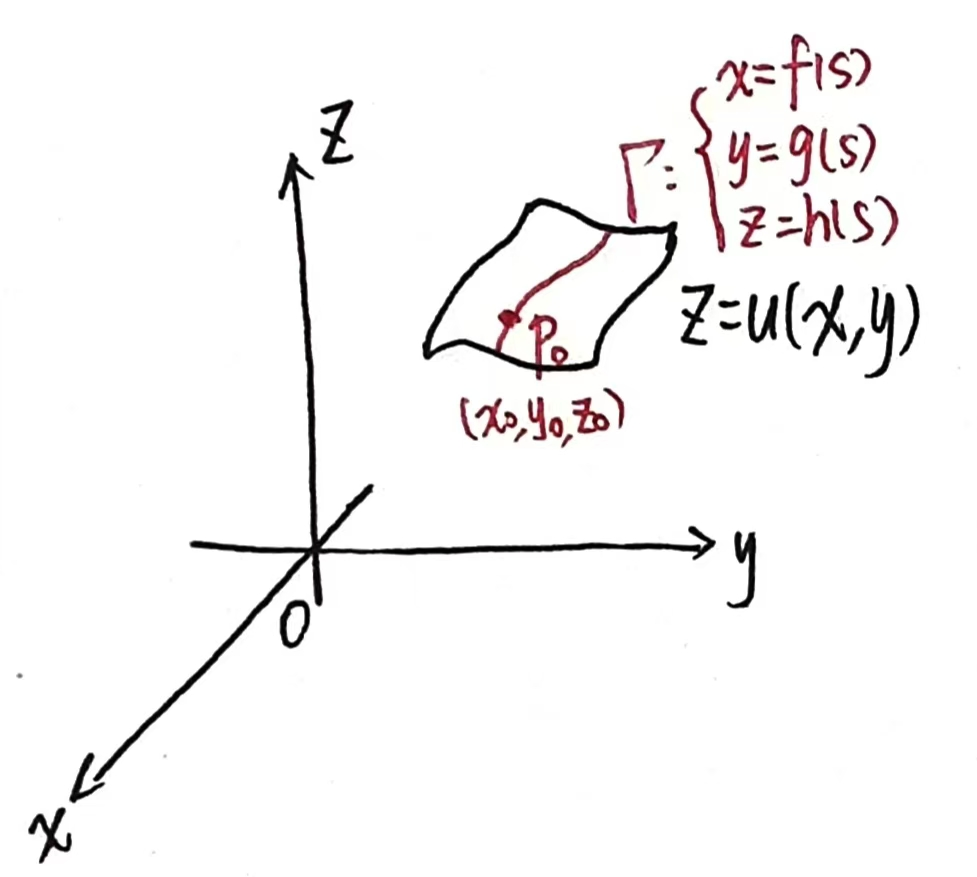
\includegraphics[width=0.4\linewidth]{figure/1.3-1}
		\caption{Cauchy Problelm for Quasi-Linear Equation}
		\label{pic : 1.3-1} % 添加图像引用标签
	\end{figure}
	
	\vspace*{2em}
	
	下面给出该Cauchy问题解存在的\textbf{充分条件}, 并将说明当已知曲线$\Gamma$ 并非点$P_0$ 处特征线时, 该条件为\textbf{充要条件}. 证明过程也即给出了运用\textbf{特征线法}求解\textbf{Quasi-Linear方程的Cauchy问题}的方法. 
	
	\newpage
	
	\begin{thm}\label{thm 1.3.1}
		\textbf{[Cauchy Problem for Quasi-Linear Equation]}. \\
		考虑如下Cauchy问题. Assume $a , b , c \in C^1$ near $P_0$. For the Quasi-Linear Equation
		\begin{align*}
			\begin{cases}
				a(x , y , u) u_x + b(x , y , u) u_y = c(x , y , u) \\
				x = f(s) , \,\, y = g(s) , \,\, z = h(s) \\
				h(s) = u \Big( f(s) , g(s) \Big) \\
				(x_0 , y_0 , z_0) = \Big( f(s_0) , g(s_0) , h(s_0) \Big)
			\end{cases}
		\end{align*}
		即已知$\R^3$ 中曲面$z = u(x , y)$ 上的一条曲线$\Gamma$ 及其上一点$P_0(x_0 , y_0 , z_0)$, 其中$\Gamma$ 的参数方程可表示为
		\begin{align*}
			\Gamma : 
			\begin{cases}
				x = f(s) \\
				y = g(s) \\
				z = h(s)
			\end{cases} , \,\, P_0 = (x_0 , y_0 , z_0) = \Big( f(s_0) , g(s_0) , h(s_0) \Big) \in \Gamma
		\end{align*}
		其中$f , g , h \in C^{1}$ near $s_0$, $s_0 \in [a , b]$. 则该Cauchy问题在$P_0$ 附近有解的\textbf{充分条件}为:
		\begin{align*}
			J = 
			\begin{vmatrix}
				f^{'}(s_0) &g^{'}(s_0) \\
				a(x_0 , y_0 , z_0) &b(x_0 , y_0 , z_0)
			\end{vmatrix}
			\neq 0
		\end{align*}
		特别地, 当$\Gamma$ 不是点$P_0$ 处的特征线时, 该条件为\textbf{充要条件}. 
		
		\vspace*{8em}
		
		\begin{proof}
			\begin{itemize}
				\item \textbf{充分性(一般情形)}:Suppose $a , b , c \in C^1(\Omega)$ and $f , g , h \in C^1[a_0 , b_0]$. \\
				Fix $s \in [a_0 , b_0]$. 对于每个$s \in [a_0 , b_0]$, 考虑如下ODE(\textbf{特征线})
				\begin{align*}
					\begin{cases}
						\dfrac{dx(t)}{dt} = a \Big( x(t) , y(t) , z(t) \Big) \\
						\dfrac{dy(t)}{dt} = b \Big( x(t) , y(t) , z(t) \Big) \\
						\dfrac{dz(t)}{dt} = c \Big( x(t) , y(t) , z(t) \Big) \\
						x(0) = f(s) , \,\, y(0) = g(s) , \,\, z(0) = h(s)
					\end{cases}
				\end{align*}
				Since $a , b , c \in C^1(\Omega)$, $f , g , h \in C^1[a_0 , b_0]$, then by \textbf{ODE解的存在唯一性定理 (Thm \ref{thm B.2.1})}, \\
				对于每个$s \in [a_0 , b_0]$, 上述ODE均有唯一解, 即对于每个$s \in [a_0 , b_0]$, 在点$P = \Big( f(s) , g(s) , h(s) \Big)$ 处均可解出唯一的一条特征线. 
				
				\newpage
				
				设所求曲面$z = u(x , y)$ 的参数方程为
				\begin{align*}
					\begin{cases}
						x = X(s , t) \\
						y = Y(s , t) \\
						z = Z(s , t)
					\end{cases}
				\end{align*}
				则将上述对于所有fixed $s \in [a_0 , b_0]$ 的ODE方程合在一起, 等价于下述ODE方程组:
				\begin{align*}
					\begin{cases}
						X_{t}(s , t) = a \Big( X(s , t) , Y(s , t) , Z(s , t) \Big) \\
						Y_{t}(s , t) = b \Big( X(s , t) , Y(s , t) , Z(s , t) \Big) \\
						Z_{t}(s , t) = c \Big( X(s , t) , Y(s , t) , Z(s , t) \Big) \\
						X(s , 0) = f(s) , \,\, Y(s , 0) = g(s) , \,\, Z(s , 0) = h(s)
					\end{cases}
				\end{align*}
				根据\textbf{ODE解的存在唯一性定理 (Thm \ref{thm B.2.1})}, 上述ODE解存在且唯一, i.e. \\
				$\exists X , Y , Z \in C^1$ near $(s_0 , 0)$, $\st$ 曲面$z = u(x , y)$ 在$P_0$ 附近参数方程为
				\begin{align*}
					\begin{cases}
						x = X(s , t) \\
						y = Y(s , t) \\
						z = Z(s , t)
					\end{cases}
				\end{align*}
				下面我们来解出曲面$z = u(x , y)$ 的表达式, 即原Quasi-Linear Equation的解:\\
				我们已知在$(s_0 , 0)$ 点附近, 
				\begin{align*}
					\begin{cases}
						x = X(s , t) \\
						y = Y(s , t)
					\end{cases}
				\end{align*}
				因为
				\begin{align*}
					\begin{vmatrix}
						X_s &X_t \\
						Y_s &Y_t
					\end{vmatrix} (s_0 , 0) 
					= 
					\begin{vmatrix}
						f^{'}(s_0) &a \Big( f(s_0) , g(s_0) , h(s_0) \Big) \\
						g^{'}(s_0) &b \Big( f(s_0) , g(s_0) , h(s_0) \Big)
					\end{vmatrix} 
					= J \neq 0
				\end{align*}
				所以根据\textbf{反函数定理 (Thm \ref{thm B.3.1})}, $\exists F , G \in C^1$ near $P_0$ 为$x = X(s , t), \,\, y = Y(s , t)$ 的反函数, $\st$
				\begin{align*}
					\begin{cases}
						s = F(x , y) \\
						t = G(x , y)
					\end{cases} 
					\,\, \Rightarrow \,\,\,\,
					z = Z(s , t) = Z\Big( F(x,  y) , G(x , y) \Big)
				\end{align*}
				Let
				\begin{align*}
					z = Z\Big( F(x , y) , G(x , y) \Big) = u(x , y)
				\end{align*}
				即得到了曲面$z = u(x , y)$ 的方程, 也即求得了原方程的解. 
				
				\newpage
				
				\item \textbf{必要性(若$\Gamma$ 并非点$P_0$处的特征线)}:反证法. Assume $J = 0$. Then 
				\[ J = b(P_0)f^{'}(s_0) - a(P_0)g^{'}(s_0) = 0 \]
				Since $h(s) = u \Big( f(s) , g(s) \Big)$ in $\Gamma$, then
				\[ h^{'}(s_0) = f^{'}(s_0) u_x + g^{'}(s_0) u_y \]
				根据原Quasi-Linear方程, 还可得到关系:
				\[ c = au_x + bu_y \]
				于是, at $s = s_0 , \,\, x = f(s_0) , \,\, y = g(s_0)$, we have three relations
				\[ bf^{'} - ag^{'} = 0 \hspace*{4em} h^{'} = f^{'}u_x + g^{'}u_y \hspace*{4em} c = au_x + bu_y \]
				These imply that\footnote{在等式$h^{'} = f^{'}u_x + g^{'}u_y$ 两侧乘$b$, 在$c = au_x + bu_y$ 两侧乘$g^{'}$, 分别得到$bh^{'} = bf^{'}u_x + bg^{'}u_y , \,\, cg^{'} = ag^{'}u_x + bg^{'}u_y$. 两个等式相减即得到$bh^{'} - cg^{'} = 0$. 同理可得到$ah^{'} - cf^{'} = 0$. }
				\[ bh^{'} - cg^{'} = 0 \,\, \text{and} \,\, ah^{'} - cf^{'} = 0 \]
				Therefore, 在$P_0$ 点, $(f^{'} , g^{'} , h^{'})$ 与$(a , b , c)$ 成比例, i.e. \\
				曲线$\Gamma$ 在点$P_0$ 处的切线方向即为$(a , b , c) \,\, \Rightarrow \,\, \Gamma$ 满足在$P_0$ 点处的特征线ODE方程. 
				
				\vspace*{1em}
				
				由\textbf{充分性}证明过程, 根据\textbf{ODE解的存在唯一性定理 (Thm \ref{thm B.2.1})}, $\Gamma$ 即为点$P_0$ 处的特征线, 这与假设条件\textbf{“$\Gamma$ 并非点$P_0$ 处的特征线”}矛盾. 
				
				\vspace*{1em}
				
				Therefore, we have proved the necessity. 
			\end{itemize}
		\end{proof}
		
		\vspace*{4em}
		
		\begin{rmk}
			可以容易地推广至\textbf{含n个自变量的1阶Quasi-Linear Equation}. 
		\end{rmk}
	\end{thm}



	%  ############################
	\ifx\allfiles\undefined
\end{document}
\fi